%%%% ijcai19.tex
\typeout{Acquiring Integer Programs from Data}

% These are the instructions for authors for IJCAI-19.

\documentclass{article}
\pdfpagewidth=8.5in
\pdfpageheight=11in
% The file ijcai19.sty is NOT the same than previous years'
\usepackage{ijcai19}

% Use the postscript times font!
\usepackage{times}
\usepackage{soul}
\usepackage{url}
\usepackage[hidelinks]{hyperref}
\usepackage[utf8]{inputenc}
\usepackage[small]{caption}
\usepackage{graphicx}
\usepackage{amsmath}
\usepackage{booktabs}
\usepackage{algorithm}
%\usepackage{algorithmic} % NOPE
\usepackage[noend]{algpseudocode}
\urlstyle{same}
% \usepackage{floatrow}

% the following package is optional:
%\usepackage{latexsym}

% Following comment is from ijcai97-submit.tex:
% The preparation of these files was supported by Schlumberger Palo Alto
% Research, AT\&T Bell Laboratories, and Morgan Kaufmann Publishers.
% Shirley Jowell, of Morgan Kaufmann Publishers, and Peter F.
% Patel-Schneider, of AT\&T Bell Laboratories collaborated on their
% preparation.

% These instructions can be modified and used in other conferences as long
% as credit to the authors and supporting agencies is retained, this notice
% is not changed, and further modification or reuse is not restricted.
% Neither Shirley Jowell nor Peter F. Patel-Schneider can be listed as
% contacts for providing assistance without their prior permission.

% To use for other conferences, change references to files and the
% conference appropriate and use other authors, contacts, publishers, and
% organizations.
% Also change the deadline and address for returning papers and the length and
% page charge instructions.
% Put where the files are available in the appropriate places.

\usepackage{amsthm,amssymb}
\usepackage{tikz}
\usepackage{tikz-qtree,tikz-qtree-compat}
\usepackage{xcolor}
\usepackage{xspace}

\newcommand{\mohit}[1]{{\bf \textcolor{blue}{{Mohit: #1}}}}
\newcommand{\luc}[1]{{\bf \textcolor{red}{{Luc: #1}}}}
\newcommand{\stefano}[1]{{\bf \textcolor{violet}{{Stefano: #1}}}}

\newcommand{\learner}{\textsc{Arnold}\xspace}
\newcommand{\acronym}{AcquiRing NOn-Linear moDels}
\newcommand{\dataset}{\ensuremath{\mathcal{D}}\xspace}
\newcommand{\tensors}{\ensuremath{\mathcal{T}}\xspace}
\newcommand{\variables}{\ensuremath{\mathcal{V}}\xspace}
\newcommand{\constants}{\ensuremath{\mathcal{C}}\xspace}
\newcommand{\indices}{\ensuremath{\mathcal{I}}\xspace}
\newcommand{\factors}{\ensuremath{\mathcal{X}}\xspace}
\newcommand{\program}{\ensuremath{\mathcal{P}}\xspace}
\newtheorem*{definition}{Definition}
\newtheorem*{example}{Example}
\newcommand{\TERM}[2]{\ensuremath{\mathrm{term}_{#1,#2}}\xspace}
\newcommand{\IDX}[1]{\ensuremath{\mathrm{index}\left(#1\right)}\xspace}
\newcommand{\RAN}[1]{\ensuremath{\mathrm{range}\left(#1\right)}\xspace}
\newcommand{\SOL}[1]{\ensuremath{\mathrm{Sol}\left(#1\right)}\xspace}
\DeclareMathOperator*{\find}{find}

\renewcommand\[{\begin{equation}}
\renewcommand\]{\end{equation}}

\newcommand{\va}{\textbf{a}\xspace}
\newcommand{\vb}{\textbf{b}\xspace}
\newcommand{\vc}{\textbf{c}\xspace}
\newcommand{\vd}{\textbf{d}\xspace}
\newcommand{\ve}{\textbf{e}\xspace}
\newcommand{\vf}{\textbf{f}\xspace}
\newcommand{\vg}{\textbf{g}\xspace}
\newcommand{\vh}{\textbf{h}\xspace}
\newcommand{\vi}{\textbf{i}\xspace}
\newcommand{\vj}{\textbf{j}\xspace}
\newcommand{\vk}{\textbf{k}\xspace}
\newcommand{\vl}{\textbf{l}\xspace}
\newcommand{\vm}{\textbf{m}\xspace}
\newcommand{\vn}{\textbf{n}\xspace}
\newcommand{\vo}{\textbf{o}\xspace}
\newcommand{\vp}{\textbf{p}\xspace}
\newcommand{\vq}{\textbf{q}\xspace}
\newcommand{\vr}{\textbf{r}\xspace}
\newcommand{\vs}{\textbf{s}\xspace}
\newcommand{\vt}{\textbf{t}\xspace}
\newcommand{\vu}{\textbf{u}\xspace}
\newcommand{\vv}{\textbf{v}\xspace}
\newcommand{\vw}{\textbf{w}\xspace}
\newcommand{\vx}{\textbf{x}\xspace}
\newcommand{\vy}{\textbf{y}\xspace}
\newcommand{\vz}{\textbf{z}\xspace}
\newcommand{\TA}{\textbf{A}\xspace}
\newcommand{\TB}{\textbf{B}\xspace}
\newcommand{\TC}{\textbf{C}\xspace}
\newcommand{\TD}{\textbf{D}\xspace}
\newcommand{\TE}{\textbf{E}\xspace}
\newcommand{\TF}{\textbf{F}\xspace}
\newcommand{\TG}{\textbf{G}\xspace}
%\newcommand{\TH}{\textbf{H}\xspace}
\newcommand{\TI}{\textbf{I}\xspace}
\newcommand{\TJ}{\textbf{J}\xspace}
\newcommand{\TK}{\textbf{K}\xspace}
\newcommand{\TL}{\textbf{L}\xspace}
\newcommand{\TM}{\textbf{M}\xspace}
\newcommand{\TN}{\textbf{N}\xspace}
\newcommand{\TO}{\textbf{O}\xspace}
\newcommand{\TP}{\textbf{P}\xspace}
\newcommand{\TQ}{\textbf{Q}\xspace}
\newcommand{\TR}{\textbf{R}\xspace}
\newcommand{\TS}{\textbf{S}\xspace}
\newcommand{\TT}{\textbf{T}\xspace}
\newcommand{\TU}{\textbf{U}\xspace}
\newcommand{\TV}{\textbf{V}\xspace}
\newcommand{\TW}{\textbf{W}\xspace}
\newcommand{\TX}{\textbf{X}\xspace}
\newcommand{\TY}{\textbf{Y}\xspace}
\newcommand{\TZ}{\textbf{Z}\xspace}


\title{Acquiring Integer Programs from Data}
\author{ID 6520}
%\author{
%Mohit Kumar$^1$,
%Stefano Teso$^1$,
%Luc De Raedt$^1$
%\\
%$^1$ KU Leuven\\
%%
%\texttt{\{mohit.kumar,stefano.teso,luc.deraedt\}@cs.kuleuven.be}
%}
% If your authors do not fit in the default space, you can increase it
% by uncommenting the following (adjust the "2.5in" size to make it fit
% properly)
% \setlength\titlebox{2.5in}

\begin{document}
\maketitle


\begin{abstract}
    Integer programming (IP) is widely used within operations research to model
    and solve complex combinatorial problems such as personnel rostering and
    assignment problems.  Modelling such problems is difficult for non-experts
    and expensive when hiring domain experts to perform the modelling.  For
    many tasks, however, examples of working solutions are readily available.
    We propose \learner, an approach that partially automates the modelling
    step by learning an integer program from example solutions.  Contrary to
    existing alternatives, \learner natively handles multi-dimensional
    quantities and non-linear operations, which are at the core of IP problems,
    and it only requires  examples of feasible solution.  The main challenge is
    to efficiently explore the space of possible programs.  Our approach pairs
    a general-to-specific traversal strategy with a nested lexicographic
    ordering in order to prune large portions of the space of candidate
    constraints while avoiding visiting the same candidate multiple times.  Our
    empirical evaluation shows that \learner can acquire models for a number of
    realistic benchmark problems.
\end{abstract}


\section{Introduction}
\label{sec:intro}

Integer programming (IP) is a widespread framework for modelling and solving
complex combinatorial problems such as scheduling, packing, routing,
\emph{etc.}~\cite{nemhauser1989integer}.  Real-world IP models consist of
multi-dimensional decision variables (e.g.  schedules) tied together by complex
constraints.
%as well as the complex constraints that hold between the variables.
Designing integer programs requires technical know-how beyond the level of
non-experts, and can be time-consuming and expensive.  This hinders the
adoption of IP.
% \luc{delete : in novel or custom settings where ready-made models are not yet
% available.}

In many applications, however, example solutions of reasonable quality are
readily available.  For instance, in nurse rostering, the hospital has access
to past nurse schedules.  In line with the previous work on constraint
acquisition~\cite{de2018learning,bessiere2017constraint,beldiceanu2012model},
we propose to partially automate the modelling process by acquiring integer
programs directly from working solutions, i.e., positive examples.

Existing approaches to constraint acquisition have not been designed to handle
this setting.  First, most of them are ill-equipped to deal with
%large numbers of decision variables,
structured (e.g. multi-dimensional) variables and non-linear constraints, which
are the norm in integer programming.  Furthermore, most of them require
examples of negative (i.e., infeasible) configurations, which are often
unavailable in applications.
%;  cf. the Related Work Section for a detailed discussion.

We contribute \learner, for \acronym, a novel approach to learn integer
programs from positive example solutions.
%
\learner relies on a tensor-based language for describing linear and non-linear
constraints between multi-dimensional quantities, which are common in integer
programs.  This representation enables handling several constraints (namely,
one per element) at once.
%
Our approach
% relies on a general-to-specific search strategy, which involves
cleverly enumerates
%(and prunes)
the potential IP constraints and collects those that are satisfied by the
example solutions.  This is guaranteed to produce a valid IP model, but it
requires the evaluation of a large number of candidates.
%
In line with approaches to inductive logic programming
\cite{de2008logical,de1997clausal} and graph mining
\cite{jiang_coenen_zito_2013}, we use two strategies to manage the enumeration
process:
%
%1)
a general-to-specific enumeration scheme that prunes away large portions of
the search space, and
%
%2)
a nested lexicographic ordering
%of the candidates
that avoidss enumerating the same constraint twice.

Summarizing, our contributions include:
%
(1) A language for describing constraints that appear in typical integer
programs,
%
(2) \learner, a novel algorithm for acquiring integer programs from examples of
feasible (but not necessarily optimal) solutions, and
%
(3) An extensive empirical analysis on a number of integer programs, showing
that \learner can acquire good quality programs from a handful of examples.


\section{Learning Integer Programs}
\label{sec:ps}

We aim to automatically acquire integer programs from positive examples.  Since
IP often relies on multi-dimensional quantities, we start  by introducing the
required notation.


\paragraph{Notation.} Scalars $x$ are written in lower-case, multi-dimensional
tensors $\TX$ in bold upper-case, and sets $\mathcal{X}$ in calligraphic
upper-case.  Given a tensor \TX, its elements are indicated as $\TX_{i,j,k}$, its indices are referred by $\IDX{\TX}$, and the ranges of those
indices as $\RAN{\TX}$.  For instance, if $\TX \in \{0,1\}^{3 \times 5}$ has indices $i$ and
$j$, then $\IDX{\TX} = \{i, j\}$ and $\RAN{\TX} = \{1, \ldots, 3\} \times \{1,
\ldots, 5\}$.

In the present paper, all operations and comparisons between tensors are
element-wise.  For instance, letting \TX and \TZ have identical dimensions,
it holds that $(\TX + \TZ)_{i,j} = \TX_{i,j} + \TZ_{i,j}$ for all $i$, $j$.
%
In IP, tensor indices often represent semantically distinct entities,
like objects to be packed or employees to be scheduled.  For this reason, when
performing operations across tensors we implicitly \emph{match indices with the
same name}.  For example, letting $\IDX{\TX}=\{i,j\}$ and
$\IDX{\TZ}=\{i,k,\ell\}$, then $\IDX{\TX \TZ} = \{i, j, k, \ell\}$ and $(\TX
\TZ)_{i,j,k,\ell} = \TX_{i,j} \TZ_{i,k,\ell}$.
%
A tensor satisfies a condition if \emph{all} of its elements satisfy that
condition, e.g., $\TX \le \TZ$ is equivalent to $\forall \, i, j, k, \ell \,.\,
\TX_{i,j} \le \TZ_{i,k,\ell}$.
%
%Finally, the indicator function $\mathbb{I}\{cond\}$ evaluates to $1$ if $cond$
%is true and to $0$ otherwise.


\paragraph{Integer programs.}  Let us introduce a toy integer program for nurse
rostering~\cite{burke2004state,smet2013nurse}.

\begin{example}
    Consider a small hospital with five nurses.  The goal is to find a seven
    day schedule, where every day has three shifts, such that a minimum number
    of at-least-medium skilled nurses are always available.
    %
    Let $\TX \in \{0, 1\}^{5 \times 7 \times 3}$ be a decision variable such
    that $\TX_{n,d,s}$ encodes whether nurse $n$ works on shift $s$ of day $d$,
    $\TV \in \{0, 1\}^5$ (resp. $\TM$, $\TL$) indicate which nurses are very
    skilled (resp. medium or low skilled), and $\TR \in \mathbb{N}^{7 \times
    3}$ be the minimum number of skilled nurses required in each shift.
    %
    Then, an integer program for this problem can be written as:
    %
    \begin{align}
        \find
            & \; \TX \nonumber
        \\
        \text{\emph{s.t.}}
            & \textstyle \; \sum_n \TV_n \TX_{n,d,s} + \sum_n \TM_n \TX_{n,d,s} \ge \TR_{d,s}
            & \forall d, s
            \label{eq:toyconst1}
    \end{align}
\end{example}

This example captures some important aspects of typical integer programs:
%
\textbf{a}) The decision variables (i.e. the quantities determined by the IP
solver, like $\TX$ above) and the constants (all the other quantities, like
$\TR$, $\TV$, $\TM$, $\TL$) are \emph{non-negative integer tensors} of
arbitrary dimensions.  We use \variables and \constants to indicate the set of
tensor variables and constants, respectively, and $\tensors =
\variables\,\cup\,\constants$ to indicate all the tensors appearing in the
program.  We stress that the constants \constants (e.g., the skill levels) are
often known beforehand.
% \stefano{their dimensions might not be?}
%
\textbf{b}) The constraints only include sums, products, and comparisons among
tensors; in other words, they are \emph{polynomial inequalities}.  The caveat
is that the variables and the value of the polynomial can be multi-dimensional.
%
\textbf{c}) The constraints are \emph{non-linear}, that is, they include
products among tensors, and potentially among decision variables.  Note that
both linear and non-linear integer programs satisfy this condition.
%
\textbf{d}) This is a \emph{satisfaction} problem.
%Many models in integer programming also have an optimisation function $F$ and
%then want to find the bets solution (w.r.t. $F$) that satisfies all the
%constraints. The current setting in which we learn from positives does not aim
%at finding such a model. One reason for this is that such a model would not
%only require positive examples that satisfy the constraints, but also examples
%that are \emph{optimal} w.r.t. the unknown function $F$. It is unrealistic
%that such optimal data points are available in any given applications. For
%instance, in real-life scheduling problems, the used schedules will be good
%enough, but there can be no guarantee that they are the best possible
%schedules.
Satisficing problems, where the goal is to find a configuration that is ``good
enough'' according to some objective function, are subsumed as a special case,
as discussed below.
%This case will be discussed in detail below.

For these reasons, we focus on IP programs \program of the form:
%
$$
    \find \; \variables \quad 
    \text{s.t.}
        \; g_j(\variables) \le \TZ_j
        \qquad j = 1, 2, \ldots, m
$$
%
where $g_1, \ldots, g_m$ are polynomials of \variables with coefficients in
\constants, and $\TZ_1, \ldots, \TZ_m$ are constants in \constants.
%
Such integer programs can be viewed as sets of polynomial constraints.  Given
\program, a \emph{solution} is a value assignment to the decision variables in
\variables that satisfies all the constraints in \program.  Abusing notation,
we write value assignments as \variables.  We use $\program \models \variables$
to indicate that a value assignment $\variables$ is feasible with respect to
\program, that is:
%
$$
    \variables \models \program \iff \forall j = 1, \ldots, m \,.\, g_j(\variables) \le \TZ_j
$$
%
We will also say that $\variables$ satisfies $P$.  The set of solutions of
$\program$ is written
$\SOL{\program} = \{\variables \,:\,  \variables \models \program\}$.

Observe that this setup also captures \emph{satisficing} scenarios, where an
(integer polynomial) objective $f(\variables)$ is given and the goal is to find
solutions satisfying $f(\variables) \ge \theta$, for some threshold $\theta$.
%Further, $\theta$ is often known to the user, e.g., the user may want schedules
%that cost less than $\theta\$$ per week.
Further, note that even pure 0--1 integer programming is extremely expressive,
as it subsumes propositional logic.

%\stefano{It also captures 0--1 cases and propositional logic.}

%\luc{The abuse of notation is a bit weird ... better to write ${\cal V}\theta$?}


\paragraph{Problem statement.} Recall that our aim is to simplify the modelling
step by acquiring a program $\program_L$ from a set of examples of feasible
solutions.  This can be formalized as follows:

\begin{definition}[Integer Program Learning]
    Given a set of tensor constants \constants, tensor decision variables
    \variables, and feasible solutions $\dataset = \{\variables_1, \ldots,
    \variables_n\}$ taken from some unknown integer program, find an integer
    program $\program_L$ that is satisfied by all  examples, i.e., $\forall i \,.\, \variables_i
    \models \program_L$.
\end{definition}

The estimated model can be used to produce new schedules that are as good or
better than the example ones.  Of course, the learned program can be validated
or extended by domains experts, for instance to include corner cases that were
not observed in the data.  At the same time, the domain experts could already
have specified  constraints that need to be part of the model $\program_L$.

Notice that we do not assume the input examples to be optimal, which would be
very hard to guarantee in practice.  Rather, we make the more realistic
assumption that they represent desirable solutions, e.g., past schedules that
were observed to work well in practice.  For instance, existing schedules are
often the result of a laborious process of trial-and-error, where a hospital's
administration tried out different alternatives and retained the ones that
worked well enough.  Of course, in general, the higher the quality of the examples, better the solutions of the learned program.


\section{Learning Integer Programs with \learner}
\label{sec:method}

We propose \learner (for \acronym), an approach for learning integer programs
that acquires polynomial constraints from examples of feasible solutions.  In
order to do so, \learner relies on a language for expressing and manipulating
the constraints, which we introduce next.

\paragraph{The constraint language.}  The basic elements of our constraints are
\emph{terms}, that is, expressions like $\sum_{d,s} \TV_n \TX_{n,d,s}$ (see
Eq.~\ref{eq:toyconst1}).  Formally, a term has the form:
%
\[
    \textstyle
    \TERM{\indices}{\factors} = \sum_{(i_1, i_2, \ldots) \in \RAN{\indices}} \prod_{\TX \in \factors} \TX_{i_1, i_2, \ldots}
    \label{eq:term}
\]
%
where $\factors \subseteq \tensors$ is a set of the decision
variables and constants appearing in the product, both of which can be a tensor. For example, in $\sum_{d,s} \TV_n \TX_{n,d,s}$, $\TV_n$ is a 1-d constant while $\TX_{n,d,s}$ is a 3-d decision variable. $\indices$ represents the set of
indices being summed over.
%
For consistency, the indices $\indices$ are required to actually appear in
the tensors in $\factors$, that is,
$\indices \subseteq \bigcup_{\TX \in \factors} \IDX{\TX}$.
%
Notice that terms are themselves multi-dimensional quantities.  In particular,
the indices of a term are the indices that appear in its tensors but are not
summed over, namely
$\IDX{\TERM{\indices}{\factors}} = \bigcup_{\TX \in \factors} \IDX{\TX} \setminus \indices$.
In the above term $\indices$ is $\{d, s\}$, which is indeed a subset of
$\{n, d, s\}$, and the term's indices are $\{n,d,s\} \setminus \{d,s\} =
\{n\}$.

The constraints we consider have the form:
%
\[
    \textstyle
    \sum_k \TERM{\indices^k}{\factors^k} \le \TZ
    \label{eq:constraint}
\]
%
As in Eq.~\ref{eq:toyconst1}, the left-hand side is a sum of
terms.  The sum implicitly iterates over all terms appearing in the constraint.
To be a \emph{well-formed} constraint, all terms in
the sum must have the same dimension.  For instance, if $\IDX{\TA} =
\IDX{\TX} = \{n,d,s\}$ and $\IDX{\TB} = \IDX{\TY} = \{n,d\}$, then $\sum_{d,s}
\TA_n \TX_{n,d,s} + \sum_d \TB_d \TY_{n,d}$ is well-formed, because
both terms have dimension $\{n\}$.  The right hand side is a single tensor
constant $\TZ \in \constants$.

Importantly, since tensor comparisons are element-wise, all of the indices that
are not summed over, namely
$\IDX{\TERM{\indices^1}{\factors^1}} \cup \IDX{\TZ}$,
are implicitly universally quantified. For example in Eq. ~\ref{eq:toyconst1},
the constraint is universally quantified over $\{d,s\}$ because
$\IDX{\textstyle \; \sum_n \TV_n \TX_{n,d,s}} \cup \IDX{\TR_{d,s}}=\{d,s\}$.
Notice that the indices of the expression on the left hand side need not be
identical to those on the right.  For instance, the constraint $\TX \le \TZ$
could have indices $\{s,n\}$ for $\TX$ and $\{s\}$ for $\TZ$, as the constraint
is universally quantified over $s$ and $n$;  in other words, this constraint
states that for all $s$ and $n$, $\TX_{s,n} \le \TZ_n$.


\begin{figure}[tb]
    \begin{center}
        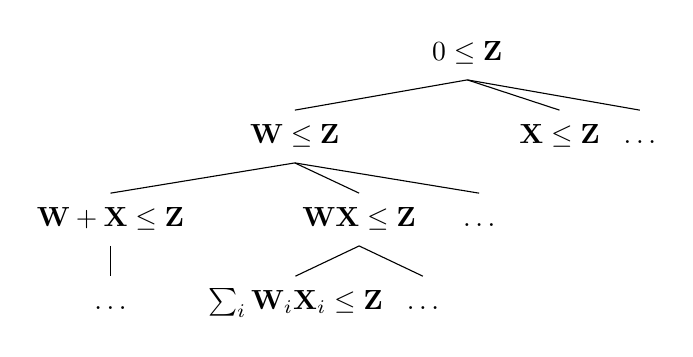
\begin{tikzpicture}[
                execute at begin node=\strut,
                level distance=3em,
            ]
%            \tikzset{grow'=right,level distance=6em}
%            \tikzset{}
%            \tikzset{every tree node/.style={anchor=base west}}
            \Tree
                [. {$0 \le \TZ$}
                    [. {$\TW \le \TZ$}
                        [.{$\TW + \TX \le \TZ$}
                            {$\ldots$}
                        ]
                        [. {$\TW \TX  \le \TZ$}
                            {$\sum_i \TW_i \TX_i \le \TZ$}
                            {$\ldots$}
                        ]
                        {$\ldots$}
                    ]
                    {$\TX \le \TZ$}
                    {$\ldots$}
                ]
        \end{tikzpicture}
        \caption{\label{fig:candidates}  Recursive refinement of a most-general
        constraint $(0 \le \TZ) \in \rho(\top)$.  The levels illustrate three
        specialization schemes: adding a term, elongating
        a product and adding an index.  All tensors $\TW$, $\TX$, $\TZ$ are non-negative and have
        single index $i$.}
    \end{center}
\end{figure}


\paragraph{The \learner algorithm.}   Given a set of feasible solutions
$\dataset = \{\variables_1, \ldots, \variables_n\}$, \learner acquires an
integer program $\program_L$ using a general-to-specific search strategy that
is reminiscent of inductive programming, graph mining and constraint
acquisition~\cite{de1997clausal,de2008logical,jiang_coenen_zito_2013,de2018learning}.

Letting $p$ be the (user-specified) maximum number of tensors in a term and $s$
the maximum number of terms in a constraint, \learner cleverly searches the
space of all syntactically correct constraints up to the given complexity and
keeps the ones that are compatible with all examples.  It is easy to see that
the number of potential terms is exponential in $p$ and that the number of
candidate constraints is even larger.  The main challenge is thus to avoid
enumerating as many candidates as possible.
%
\learner adopts two strategies to prune the search space:
%
1) Enumerating the candidate constraints in a general-to-specific fashion,
which allows it to prune away large parts of the search space; and
%
2) Using a canonical form and a nested lexicographic ordering to avoid enumerating
the same constraint twice.
%
%In this sense, \learner is similar to the clausal discovery algorithm
%\cite{de1997clausal}, which searches for clauses (logical constraints) that
%hold in the data rather than IP contraints.

%\luc{probably good to list all our assumption in this intro already?}


\paragraph{General-to-specific search.} Given two constraints $c$ and $c'$, we
say that $c$ is more specific than $c'$ (and that $c'$ is more general than
$c$), written $c \models c'$, if and only if all value assignments \variables
that satisfy $c$ also satisfy $c'$.  Intuitively, specializations impose more
strong conditions in the left hand side of the constraint.  For instance, if
$\TP$ is non-negative, then $(\TX + \TP \le \TZ) \models (\TX \le \TZ)$ holds
for any $\TX$, $\TZ$ of compatible sizes.
%
Enumerating constraints in a general-to-specific order is convenient because,
whenever a constraint $c$ is inconsistent with the examples \dataset, all of
the more specific constraints $c'$ are also inconsistent and can be efficiently
pruned.
%
This is in line with logical and relational learning, where the generality
relation coincides with logical entailment~\cite{de2008logical}.

As in that line of work, \learner performs general-to-specific search by
recursively specializing constraints using a \emph{refinement operator}.  A
refinement operator $\rho$ maps a constraint $c$ (or a set of constraints) to a
set of more specific constraints $\rho(c)$.  A complete general-to-specific
search then starts from the maximally general
%element in the search space
constraint (denoted by $\top$), and recursively applies the refinement operator
$\rho$, while imposing some pruning.% \luc{as in Algorithm, 1}. 
The recursive application of a refinement
operator $\rho$ is denoted by $\rho^n$ if it is applied recursively $n$ times.
Furthermore, $\rho^*(c) = \rho(c) \cup \rho^2(c) \cup \ldots$

\learner follows this schema faithfully, see Algorithm~\ref{alg:arnold}.  In
particular, \learner uses an \emph{ad hoc} refinement operator for generating
polynomial integer programming constraints, discussed next.  In order to
simplify the presentation, we temporarily assume all tensors to be
non-negative, i.e., for all $\TX \in \tensors$, $\TX \ge 0$.  Notice that, in
this case, the most general constraints are simply $\rho(\top) = \{0 \le \TZ
\,:\, \TZ \in \tensors\}$.
%, where $\top$ is an artificial constraint, added for convenience of notation.


\begin{algorithm}[tb]
    \begin{algorithmic}[1]
        \Procedure{\learner}{$\dataset$: dataset}
            \State \Return \textsc{Refine}($\top$, \dataset)
        \EndProcedure
        %\Statex
        \Procedure{Refine}{$c$: constraint, \dataset}
            \State $\program_c \gets \emptyset$
            \If{$\dataset \models c$}
                \State $\program_c \gets \{c\}$
                \For{$c' \in \rho(c)$}
                    \State $\program_c \gets \program_c \cup \textsc{Refine}(c', \dataset)$
                \EndFor
            \EndIf
            \State \Return $\program_c$
        \EndProcedure
    \end{algorithmic}
    \caption{\label{alg:arnold} The \learner search algorithm.}
\end{algorithm}


\paragraph{The refinement operator.}  We are now ready to define our refinement
operator.
%
In this definition, we distinguish
%
% \emph{non-negative} tensors satisfying $\TP \ge 0$,
%
% \emph{non-positive} tensors satisfying $\TN \le 0$,
%
\emph{good} tensors satisfying $\TG \ge 1$,
%
\emph{bad} tensors satisfying $0 \le \TB \le 1$,
%
and \emph{ugly} tensors $\TU$, which are neither good nor bad.
%
All the other unqualified (but still positive) tensors will be denoted by
$\TX$, $\TY$, $\TZ$.
%
Let $c$ be a well-formed constraint
$\sum_k \TERM{\indices^k}{\factors^k} \le \TZ$
and
$\TERM{\indices^\ell}{\factors^\ell}$
be one of its terms.  All specializations $c' \in \rho(c)$ are obtained by
increasing the left hand side of $c$ through any of the following operations:

a) \emph{Adding a term to the left hand side.}  For every non-negative tensor
$\TP \in \tensors$, adding it as a term:
%
$$
    \textstyle
    \sum_k \TERM{\indices^k}{\factors^k} + \TP \ge \sum_k \TERM{\indices^k}{\factors^k}
$$
%
% This has the effect of tightening the inequality.

b) \emph{Adding an index to a term.}  For any non-negative term
$\TERM{\indices^\ell}{\factors^\ell} \ge 0$, adding another index $i$ to
$\indices^\ell$, that is:
%
$$
    \textstyle
    \TERM{\indices^\ell \cup \{i\}}{\factors^\ell} \ge \TERM{\indices^\ell}{\factors^\ell}
$$
%
For instance, consider a $2 \times 2$ non-negative tensor tensor $\TP$ with
indices $\{i, j\}$.  Then, the sum
$\sum_{i,j} \TP_{i,j} = \TP_{1,1} + \ldots + \TP_{1,2}$
is always (element-wise) greater than or equal to the partial sums
$\sum_i \TP_{i,j} = (\TP_{1,1} + \TP_{1,2}, \TP_{2,1} + \TP_{2,2})$
and
$\sum_j \TP_{i,j} = (\TP_{1,1} + \TP_{1,2}, \TP_{2,1} + \TP_{2,2})$.

c) \emph{Adding a tensor to a product.}  For any non-negative term
$\TERM{\indices^\ell}{\factors^\ell} \ge 0$, adding any good tensor $\TG \in
\tensors$ to a product:
%
$$
    \textstyle
    \TERM{\indices^\ell}{\factors^\ell \cup \{\TG\}} \ge \TERM{\indices^\ell}{\factors^\ell}
$$
%
It is easy to verify that, for every $c'$ above, $c' \models c$.

Notice that none of the above operations changes the right hand side of $c$:
doing so would amount to replacing the tensor $\TZ$ with some other tensor.
However, all valid alternatives are already implicitly enumerated when
contructing $\rho(\top)$.


\paragraph{Dealing with bad tensors.}  For bad tensors, which have elements
between $0$ and $1$, cases (a) and (b) are still valid, but case (c) is not.
Indeed, adding a bad tensor to a product reduces the value of the LHS, rather
than increasing it.  The refinement operator has to be extended with:

d) \emph{Removing a bad tensor from a product.}   Removing a bad tensor $\TB$
from any term $\TERM{\indices^\ell}{\factors^\ell} \ge 0$:
%
$$
    \textstyle
    \TERM{\indices^\ell}{\factors^\ell \setminus \{\TB\}} \ge \TERM{\indices^\ell}{\factors^\ell}
$$

Now, two desirable properties of refinement operators in our context are:
%
\emph{completeness}, i.e., $\rho^*(\top)$ corresponds to the set of all
well-formed constraints; and
%
\emph{non-redundancy}, in that for every well-formed constraint $c$ there is
exactly one sequence of constraints $c_1, \ldots , c_n$ such that $c_1 \in
\rho(\top), c_2 \in \rho(c_1), \ldots, c \in \rho(c_n)$.
%
%Ideal operators ensure that the same constraint is never generated multiple
%times.  This is often realized by using a lexicographic order to define a
%canonical form.
%
To ensure that our refinement operator is complete, it should always increase
the left hand side of $c$ by the tiniest possible amount.  When bad tensors are
considered, the minimal increase is obtained by multiplying together $p - 1$
bad tensors, namley $\TB_1 \cdot \ldots \cdot \TB_{p-1}$.  Consequently, case
(a) has to be revised as follows:

a') \emph{Adding a non-negative term to the LHS.}  For every non-negative
tensor $\TP \in \tensors$, adding $\TP \prod_{i=1}^{p-1}\TB_i$, that is:
%
$$
    \textstyle
    \sum_k \TERM{\indices^k}{\factors^k} + \TP \prod_{i=1}^{p-1}\TB_i \ge \sum_k \TERM{\indices^k}{\factors^k}
$$
Of course, in the absence of bad tensors (a) and (a') coincide.


\paragraph{Dealing with ugly tensors.}  Unlike good or bad tensors, multiplying
a term with an ugly tensor neither specializes nor generalizes the constraint.
Therefore, we cannot define an operation for $\rho$ to add an ugly tensor to a
product.  Instead, for each constraint produced by the refinement operation, we
\emph{manually} generate constraints by adding an ugly tensor to any term in
the left hand side.  We then perform general-to-specific search on the
resulting constraints.


% \stefano{extremely unclear:}\luc{indeed}
% So, the first two refinement operators defined above \luc{which are a and b?} would produce constraints
% with ugly tensors in summations but the multiplicative operators corresponding
% to good and bad tensors would miss out the constraints where ugly tensors are
% multiplied to a term.  To include these, for each node we consider all possible
% nodes obtained by multiplying a term in the constraint with an ugly tensor and
% include it in the enumeration process.


\paragraph{Nested lexicographic ordering.}  Notice that our refinement operator
$\rho$ is not optimal, as distinct constraints $c_1$ and $c_2$ can have the
same specialization $c'$.  For instance, if $\tensors = \{\TX, \TY, \TZ\}$,
then $\TX + \TY \le \TZ$ can be obtained by specializing either $\TX \le \TZ$
or $\TY \le \TZ$.  In this case, $c'$ and all of its descendants would be
enumerated twice.

To avoid this situation, we define a nested lexicographic ordering over
\emph{tensors}, \emph{indices}, \emph{terms} and \emph{operations} used for
refinement in the following way:
%
(1) $\rho(c)$ can only use operations of higher or equal lexical rank compared
to the operations used to reach $c$ from a most general constraint;
%
(2) $\rho(c)$ can only modify a term of higher or equal lexical rank compared
to the terms modified in $c$; and
%
(3) $\rho(c)$ can only add or remove tensors (resp. indices) from a term that
have higher or equal lexical order compared to the tensors (resp. indices)
added or removed from that term previously.

For tensors and indices we used standard alphabetical order.  For terms, the
one added last has the highest order, so that $\rho$ can modify it.
For operations, using the wrong order can make enumeration skip over some
constraints.  For example, in an ordering where (b) $\preceq$ (a'), after
adding a term we can not sum it over any index.  To ensure the completeness of
the refinement operator we define the following ordering: (a') $\preceq$ (d)
$\preceq$ (c) $\preceq$ (b).  The intuition is that:
%
(a') $\preceq$ (d), because a bad tensors must be added to a term before it can
be removed;
%
(d) $\preceq$ (c), since terms added by (a') have $p$ tensors, we
allow (d) to remove them before allowing (c) to add more;
%
(c) $\preceq$ (b), since operators preceding (b) make changes to a term, we
allow (b) to add indexes to any of these modified terms.


\paragraph{Dealing with negative tensors.}  A side-effect of only allowing
non-negative tensors is that constraints like $\sum_{i,j} X_{i,j} \ge \TZ$, or
equivalently $-\sum_{i,j} X_{i,j} \le -\TZ$, can not be represented.  This can
be fixed by allowing both non-positive and non-negative tensors.  Doing so
amounts to factorizing the sign out of the tensors themselves and into the
terms and constraints in Eq.~\ref{eq:term}--\ref{eq:constraint}, thus updating
them to:
%
\begin{align*}
    \textstyle
    \TERM{\indices}{\factors}
        & \; \textstyle = \pm \sum_{(i_1, i_2, \ldots) \in \RAN{\indices}} \prod_{\TX \in \factors} \TX_{i_1, i_2, \ldots}
    \\
    \textstyle
    \sum_k \TERM{\indices^k}{\factors^k}
        & \; \textstyle \le \pm \TZ
\end{align*}
%
In doing so, we can safely assume that all tensors in $\tensors$ are
non-negative, w.l.o.g.
%
The refinement operator must be adapted accordingly.  Most importantly,
$\rho(\top)$ now contains all constraints with the most negative possible left
hand side, i.e., the sum of the most negative terms that can be built with the
tensors in $\tensors$.
%
We add four more operations in $\rho$ to deal with negative terms. Each of
these are analogous to the operations defined above. For example, similar to
(a), removing a negative term from the left hand side of a constraint $c$
produces a more specific constraint.  The complete list is:
% Second, it leads to some added refinement operations. Let $c = ( \sum_k
% \TERM{\indices^k}{\factors^k} \le \TZ )$ be a well-formed constraint. We add
% the following refinement operators:\luc{we are actually defining one
% refinement operator, using many different types of refinement operations ...
% }
% \luc{Other complication ? we could get $X + Y < Z $ is equivalent to $X - Z <
% -Y$ Generated twice ?}
e) \emph{Removing a non-positive term from the LHS.}
    % Removing a
    %     non-positive term $\TN$ appearing in $c$ increases the value, so we
    %     take:
    %     %
    %     $$
    %         \textstyle
    %         c' = \left( \sum_k \TERM{\indices^k}{\factors^k} - \TN \le \TZ \right)
    %     $$
f) \emph{Removing an index from a non-positive term.}
    % For any
    %     non-positive term $\TERM{\indices^\ell}{\factors^\ell} \le 0$ in $c$,
    %     removing any index $i'$ appearing in $\indices^\ell$ increases the
    %     LHS.
    %     $$
    %         \textstyle
    %         c' = \left( \sum_{k \ne \ell} \TERM{\indices^k}{\factors^k} + \TERM{\indices^\ell \setminus \{i'\}}{\factors^\ell} \le \TZ \right)
    %     $$
    %     For example, if $\TN \le 0$ is $2 \times 2$ with indices $\{i, j\}$, then
    %     $\sum_{i,j} \TN_{i,j}$ is always less than or equal to any of its
    %     partial sums.
        %
g) \emph{Removing a good tensor from a non-positive term.}
        % Vice-versa, removing a good tensor from a non-positive term $\TERM{\indices^\ell}{\factors^\ell} \le 0$ in $c$ also increases the LHS
        % %
        % $$
        %     \textstyle
        %     c' = \left( \sum_{k=1}^{K-1} \TERM{\indices^k}{\factors^k} - \TERM{\indices^K}{\factors^K \setminus \{\TG'\}} \le \TZ \right)
        % $$
        % \item[d)] \emph{Multiplying a bad tensor to a non-positive term.}   For every bad tensor $\TB' \in
        % \tensors$, the constraint $c'$ obtained by elongating a product with
        % $\TB'$:
        % $$
        %     \textstyle
        %     c' = \left( \sum_{k=1}^{K-1} \TERM{\indices^k}{\factors^k} - \TERM{\indices^K}{\factors^K \cup \{\TB'\}} \le \TZ \right)
        % $$
h) \emph{Multiplying a bad tensor to a non-positive term.}
\noindent
%\paragraph{Discussion} \stefano{discuss properties of our operator}
%\begin{itemize}
%
%    \item First, the most general are generated by:
%        %
%        \textbf{a}) Picking the right hand side tensor $\TZ$ from \tensors;
%        %
%        \textbf{b}) Generating all left-hand side tensors $\TX$ from \tensors.
%
%        Create all possible configurations for LHS such that all the signatures
%        are satisfied and the value is minimum.  \luc{What do you mean by value
%        is minimum?} There can be multiple configurations that satisfy these
%        properties. For example, consider the nurse rostering example defined
%        above, if the signature specifies $m = 2$ and $n = 2$, some of the
%        possible configurations for LHS would be:
%        %
%        $-\sum_{n,d,s} \textbf{H}_n \TX_{n,d,s} - \sum_{n,d,s} \textbf{M}_n \TX_{n,d,s}$, $-\sum_{n} \textbf{H}_n \textbf{H}_{n} - \sum_{n,d,s} \textbf{M}_n \TX_{n,d,s}$
%
%    \item For every root, recursively check its trees. \luc{Subtress ? still
%    need to be generated ... searched}  Thereafter children are generated for
%    each root by keeping \TZ fixed and increasing the value for LHS by using
%    operations and conditions on tensor that guarantee the entailment
%    property.
%
%\end{itemize}
% In the procedure \textsc{BuildTree}, first all the possible root nodes are
% generated, for each root if it either does not satisfy the signatures or
% satisfies the constraint we enumerate the possible tree from that root node.
% When a node doesn't satisfy the signatures the constraint represented by it
% doesn't make sense and hence can't be verified but a child of such node might
% satisfy the signatures and the constraint represented as well. Hence, while
% enumerating the constraint entailment tree, children are generated for a node
% only if either it doesn't satisfy the signatures or satisfies the constraint.
%
% In the $enumerate$ procedure we use a depth first search, for each node
% children are generated unless the node satisfies the signature but not the
% constraint, if none of it's children satisfy the constraint only then that
% node is included in the constraint list. There are two important functions
% used in this algorithm, one is $generateRoots$ and the other is
% $generateChildren$. We have already seen earlier how to generate roots, let
% us see now how to generate children.
% \begin{proposition}
% Using the ordering of tensors, dimensions and operations defined above we can
% enumerate all possible constraints in $\mathcal{C}$
% \end{proposition}
% \begin{proof}
% All terms can be divided into 7 types based on what type of tensors are
% present in it: (1) terms with only good tensors, (2) Terms with only bad
% tensors, (3) Terms with only ugly tensors, (4) Terms with only good and bad
% tensors, (5) Terms with only good and ugly tensors, (6) Terms with only bad
% and ugly tensors and finally (7) Terms with all three types of tensor good,
% bad and ugly in it.
% For all $\TT \in \TC \in \mathcal{C}$
% % The complete list of operations defined in the bad tensor section can be
% divided into two parts, the first four are on negative terms while the last
% four are on the positive terms, if we reverse these operations meaning that
% perform the first four on the positive terms while the last four on the
% negative ones, we get a
% % We can notice that all the operations we have defined to generate children
% increase the LHS, while for root nodes are defined in a way such that doing
% none of the defined operations when performed on them can decrease their
% value while satisfying the signatures
% \end{proof}
% \subsection{Bringing it all together}
% We will use the bottom up approach, so we start with the most specific
% constraint and if it's satisfied we consider all it's children and if not we
% remove it and all it's descendants, we will define a total ordering on the
% set of constraints to remove redundancy when enumerating as multiple nodes
% can have same children. To define ordering we are going to separate
% Eq~\ref{eq:constraint}: the positive one and the negative one.
% \\
% A positive term can be made more general by doing one of the following:
% \begin{itemize}
% \item $|E'| > |E|$, adding more positive terms
% \item $\exists l'\in E \quad s.t. \quad  |l'| < |l|$, adding more products
% \item $\exists S'_l\in E \quad s.t. \quad S'_l \subset S_l$, summing over more dimensions
% \end{itemize}
% A negative term can be made more general by doing one of the following:
% \begin{itemize}
% \item $|F'| < |F|$, removing negative terms
% \item $\exists l'\in F \quad s.t. \quad  |l'| > |l|$, removing products
% \item $\exists S'_l\in F \quad s.t. \quad S'_l \supseteq S_l$, summing over less dimensions
% \end{itemize}
% We define a node $n'$  to be a child of another node $n$ if and only if either $n'$ has a positive node that is child of another positive node in $n$ or $n'$ has a negative node that is child of another negative node in $n$ but never both.
We define an ordering for these added operations which is just the opposite of the order defined for the analogous operations earlier. For example, previously it made sense to add a term before adding an index to that term. Similarly, now it makes sense to remove an index from a term before removing the term. 
The complete ordering of operations used is given by: (f) $\preceq$ (g) $\preceq$ (h) $\preceq$ (e) $\preceq$ (a') $\preceq$ (d)
$\preceq$ (c) $\preceq$ (b). Notice that the operations for non-positive terms precedes the ones for non-negative terms because the LHS in $\rho(\top)$ starts with all negative terms.

\noindent
To make sure that $\rho(c)$ produces well formed constraints we make sure that it only add terms which are compatible with sum (i.e., dimensions of terms must be same). The refinement operators produce all possible constraints as long as we are dealing with good and bad tensors. The constraints with ugly tensors are enumerated separately as discussed in the above section. Optimality is only guaranteed for the case when we have positive terms with good tensors.

\section{Empirical Analysis}

We addressed the following research questions\footnote{The experiments are
available at: \texttt{url anonymized}.}:
%
\textbf{Q1}) Does \learner acquire accurate integer programs?
%
\textbf{Q2}) Is \learner efficient in practice?
%
\textbf{Q3}) Do pruning and nested lexicographic ordering reduce the runtime of
\learner?
%
To this end, we used \learner for learning 10 satisfaction/satisficing
MiniZinc~\cite{nethercote2007minizinc} benchmark integer programs\footnote{From
\texttt{github.com/MiniZinc/benchmarks} and from the operations research
category of \texttt{hakank.org/minizinc}.}, detailed in
Table~\ref{tab:problems}.  To make sure that the learning task is challenging
enough, we chose programs with at least 5 tensors.


\begin{figure*}
\centering
\begin{minipage}{0.25\linewidth}
\centering
\includegraphics[width=\linewidth]{"images/naive_comparision_Avg Time".png}
 \includegraphics[width=\linewidth]{"images/naive_comparision_Avg Constraints".png}
\caption{\label{fig:results}  Effect of general-to-specific pruning and
    nested lexicographic ordering.  Top: average runtime (and variance) for
    $s=1$ and $p = 1, 2, 3$ (logarithmic scale - base 10).  Bottom: average number of
    acquired constraints (logarithmic scale).  (Best viewed in color.)}
\end{minipage}
\hspace{0.3 cm}
\begin{minipage}{0.70\linewidth}
\centering
\captionsetup{type=table} %% tell latex to change to table
% \begin{table*}[tb]
    % \centering
    \begin{small}
    \begin{tabular}{l|r|r|rr|rr}
        \textbf{Problem}\;$\program_*$  & $n$   & $s,p=1,1$   & $s,p=1,2$       & $s,p=1,3$           & $s,p=2,1$       & $s,p=3,1$       \\
        \toprule
        knapsack                        & 1     & $0.70,\; 0.12$  & $0.54, \; \textbf{1.00}$ & $0.49, \; \textbf{1.00}$  & $0.20, \; 0.20$   & $0.11, 0.20$  \\
                                        & 25    & $\textbf{0.99},\; 0.09$  & $\textbf{0.97}, \; \textbf{1.00}$ & $\textbf{0.96}, \; \textbf{1.00}$  & $\textbf{0.96}, \; 0.30$   & $\textbf{0.92}, 0.32$  \\
        \midrule
        shipping                        & 1     & $\textbf{1.00},\; \textbf{1.00}$  & $0.01, \; \textbf{1.00}$ & $0.80, \; \textbf{1.00}$  & $\textbf{1.00}, \; \textbf{1.00}$   & $\textbf{1.00}, \textbf{1.00}$  \\
                                        & 25    & $\textbf{1.00},\; \textbf{1.00}$  & $0.01, \; \textbf{1.00}$ & $\textbf{1.00}, \; \textbf{1.00}$  & $\textbf{1.00}, \; \textbf{1.00}$   & $\textbf{1.00}, \textbf{1.00}$  \\
        \midrule
        assignment                      & 1     & $0.49,\; 0.03$  & $0.19, \; \textbf{1.00}$ & $0.11, \; \textbf{1.00}$  & $0.16, \; 0.06$   & $0.06, 0.10$  \\
                                        & 25    & $\textbf{0.98},\; 0.01$  & $\textbf{0.98}, \; \textbf{1.00}$ & $\textbf{0.98}, \; \textbf{1.00}$  & $\textbf{0.98}, \; 0.03$   & $\textbf{0.97}, 0.03$  \\
        \midrule
        capital-                  & 1     & $0.36,\; 0.01$  & $0.06, \; \textbf{1.00}$ & $0.01, \; \textbf{1.00}$  & $0.03, \; 0.04$   & $0.01, 0.10$  \\
                                       budget & 25    & $\textbf{0.96},\; 0.01$  & $\textbf{0.95}, \; \textbf{1.00}$ & $\textbf{0.91}, \; \textbf{1.00}$  & $\textbf{0.92}, \; 0.00$   & $\textbf{0.91}, 0.01$  \\
        \midrule
        stuckey-              & 1     & $0.35,\; 0.03$  & $0.10, \; \textbf{1.00}$ & $0.10, \; \textbf{1.00}$  & $0.24, \; 0.76$   & $0.13, 0.03$  \\
                                      assignment  & 25    & $\textbf{1.00},\; 0.01$  & $\textbf{0.98}, \; \textbf{1.00}$ & $\textbf{0.98}, \; \textbf{1.00}$  & $\textbf{0.98}, \; 0.09$   & $\bullet$     \\
        \midrule
        schedule                        & 1     & $\textbf{1.00},\; 0.00$  & $\textbf{0.95}, \; 0.00$ & $0.20, \; 0.72$  & $\textbf{1.00}, \; \textbf{1.00}$   & $\textbf{1.00}, \textbf{1.00}$  \\
                                        & 25    & $\textbf{1.00},\; 0.00$  & $\textbf{0.98}, \; 0.00$ & $\textbf{0.97}, \; 0.00$  & $\textbf{1.00}, \; \textbf{1.00}$   & $\bullet$     \\
        \midrule
        curriculum                      & 1     & $0.82,\; 0.00$  & $0.27, \; \textbf{1.00}$ & $0.08, \; \textbf{1.00}$  & $0.02, \; 0.00$     & $\bullet$     \\
                                        & 25    & $\textbf{1.00},\; 0.00$  & $\textbf{0.96}, \; \textbf{1.00}$ & $\textbf{0.96}, \; \textbf{1.00}$  & $0.93, \; 0.00$     & $\bullet$     \\
        \midrule
        scheduling-                & 1     & $0.02,\; 0.04$  & $0.04, \; 0.40$ & $0.00, \; 0.50$  & $0.00, \; \textbf{1.00}$   & $0.00, \textbf{1.00}$  \\
                                      bratko  & 25    & $\textbf{1.00},\; 0.00$  & $\textbf{0.92}, \; 0.00$ & $\textbf{0.91}, \; 0.00$  & $\textbf{0.90}, \; \textbf{1.00}$   & $\bullet$     \\
        \midrule
        social-                   & 1     & $\textbf{1.00},\; 0.00$  & $0.71, \; 0.00$ & $0.68, \; 0.00$  & $\textbf{0.91}, \; 0.00$   & $\textbf{0.91}, 0.00$  \\
                                       golfers & 25    & $\textbf{1.00},\; 0.00$  & $\textbf{1.00}, \; 0.00$ & $\textbf{0.98}, \; 0.00$  & $\textbf{0.98}, \; 0.00$   & $\textbf{0.98}, 0.00$  \\
        \midrule
        rostering                       & 1     & $\textbf{1.00},\; 0.00$  & $0.87, \; 0.00$ & $0.65, \; 0.00$  & $\textbf{1.00}, \; 0.00$   & $\textbf{1.00}, 0.00$  \\
                                        & 25    & $\textbf{1.00},\; 0.00$  & $\textbf{1.00}, \; 0.00$ & $\textbf{0.99}, \; 0.00$  & $\textbf{1.00}, \; 0.00$   & $\bullet$     \\
        \bottomrule
    \end{tabular}
    \end{small}
    \caption{\label{tab:results}  Cells report the average (recall, precision)
    of the program learned by \learner; $n$, $s$, and $p$ are as in the main
    text.  Bold indicates values above while $90\%$, $\bullet$ represents time-outs.}
% \end{table*}
\end{minipage}
\end{figure*}


\begin{table}[tb]
    \begin{center} \begin{small}
        \begin{tabular}{lcccccc}
            \textbf{Problem}\;$\program_*$ & $|\variables|$ & $|\constants|$ & Largest  & $\#G$ & $\#B$ & $\#U$ \\
            \toprule
            knapsack                        & $1$  & $4$ & $5 \times 1$ & $4$ & $0$ & $1$\\
            shipping                        & $1$  & $4$ & $4 \times 3$ & $4$ & $0$ & $1$\\
            social golfers                  & $1$  & $5$ & $9 \times 4$ & $6$ & $0$ & $0$\\
            assignment                      & $2$  & $4$ & $5 \times 4$ & $5$ & $1$ & $0$\\
            capital budget                  & $2$  & $5$ & $4 \times 1$ & $6$ & $0$ & $1$\\
            stuckey assignment              & $2$  & $5$ & $5 \times 5$ & $6$ & $1$ & $0$\\
            schedule                        & $3$  & $5$ & $7 \times 1$ & $8$ & $0$ & $0$\\
            rostering                       & $3$  & $5$ & $7 \times 3$ & $8$ & $0$ & $0$\\
            curriculum                      & $3$  & $7$ & $46 \times 8$ & $9$ & $1$ & $0$\\
            scheduling bratko               & $5$  & $6$ & $1 \times 1$ & $10$ & $1$ & $0$\\
            \bottomrule
        \end{tabular}
    \end{small} \end{center}
    \caption{\label{tab:problems} Properties of the problems used in
    the experiments, including (left to right): number of variables, number of
    constants, size of the largest tensor, and number of good/bad/ugly
    tensors.}
\end{table}


% \begin{table*}[tb]
%     \centering
%     \begin{small}
%     \begin{tabular}{l|r|r|rr|rr}
%         \textbf{Problem}\;$\program_*$  & $n$   & $(s,p) = (1,1)$   & $(1,2)$       & $(1,3)$           & $(2,1)$       & $(3,1)$       \\
%         \toprule
%         knapsack                        & 1     & $0.70,\; 0.12$  & $0.54, \; \textbf{1.00}$ & $0.49, \; \textbf{1.00}$  & $0.20, \; 0.20$   & $0.11, 0.20$  \\
%                                         & 25    & $\textbf{0.99},\; 0.09$  & $\textbf{0.97}, \; \textbf{1.00}$ & $\textbf{0.96}, \; \textbf{1.00}$  & $\textbf{0.96}, \; 0.30$   & $\textbf{0.92}, 0.32$  \\
%         \midrule
%         shipping                        & 1     & $\textbf{1.00},\; \textbf{1.00}$  & $0.01, \; \textbf{1.00}$ & $0.80, \; \textbf{1.00}$  & $\textbf{1.00}, \; \textbf{1.00}$   & $\textbf{1.00}, \textbf{1.00}$  \\
%                                         & 25    & $\textbf{1.00},\; \textbf{1.00}$  & $0.01, \; \textbf{1.00}$ & $\textbf{1.00}, \; \textbf{1.00}$  & $\textbf{1.00}, \; \textbf{1.00}$   & $\textbf{1.00}, \textbf{1.00}$  \\
%         \midrule
%         assignment                      & 1     & $0.49,\; 0.03$  & $0.19, \; \textbf{1.00}$ & $0.11, \; \textbf{1.00}$  & $0.16, \; 0.06$   & $0.06, 0.10$  \\
%                                         & 25    & $\textbf{0.98},\; 0.01$  & $\textbf{0.98}, \; \textbf{1.00}$ & $\textbf{0.98}, \; \textbf{1.00}$  & $\textbf{0.98}, \; 0.03$   & $\textbf{0.97}, 0.03$  \\
%         \midrule
%         capital budget                  & 1     & $0.36,\; 0.01$  & $0.06, \; \textbf{1.00}$ & $0.01, \; \textbf{1.00}$  & $0.03, \; 0.04$   & $0.01, 0.10$  \\
%                                         & 25    & $\textbf{0.96},\; 0.01$  & $\textbf{0.95}, \; \textbf{1.00}$ & $\textbf{0.91}, \; \textbf{1.00}$  & $\textbf{0.92}, \; 0.00$   & $\textbf{0.91}, 0.01$  \\
%         \midrule
%         stuckey assignment              & 1     & $0.35,\; 0.03$  & $0.10, \; \textbf{1.00}$ & $0.10, \; \textbf{1.00}$  & $0.24, \; 0.76$   & $0.13, 0.03$  \\
%                                         & 25    & $\textbf{1.00},\; 0.01$  & $\textbf{0.98}, \; \textbf{1.00}$ & $\textbf{0.98}, \; \textbf{1.00}$  & $\textbf{0.98}, \; 0.09$   & $\bullet$     \\
%         \midrule
%         schedule                        & 1     & $\textbf{1.00},\; 0.00$  & $\textbf{0.95}, \; 0.00$ & $0.20, \; 0.72$  & $\textbf{1.00}, \; \textbf{1.00}$   & $\textbf{1.00}, \textbf{1.00}$  \\
%                                         & 25    & $\textbf{1.00},\; 0.00$  & $\textbf{0.98}, \; 0.00$ & $\textbf{0.97}, \; 0.00$  & $\textbf{1.00}, \; \textbf{1.00}$   & $\bullet$     \\
%         \midrule
%         curriculum                      & 1     & $0.82,\; 0.00$  & $0.27, \; \textbf{1.00}$ & $0.08, \; \textbf{1.00}$  & $0.02, \; 0.00$     & $\bullet$     \\
%                                         & 25    & $\textbf{1.00},\; 0.00$  & $\textbf{0.96}, \; \textbf{1.00}$ & $\textbf{0.96}, \; \textbf{1.00}$  & $0.93, \; 0.00$     & $\bullet$     \\
%         \midrule
%         scheduling bratko               & 1     & $0.02,\; 0.04$  & $0.04, \; 0.40$ & $0.00, \; 0.50$  & $0.00, \; \textbf{1.00}$   & $0.00, \textbf{1.00}$  \\
%                                         & 25    & $\textbf{1.00},\; 0.00$  & $\textbf{0.92}, \; 0.00$ & $\textbf{0.91}, \; 0.00$  & $\textbf{0.90}, \; \textbf{1.00}$   & $\bullet$     \\
%         \midrule
%         social golfers                  & 1     & $\textbf{1.00},\; 0.00$  & $0.71, \; 0.00$ & $0.68, \; 0.00$  & $\textbf{0.91}, \; 0.00$   & $\textbf{0.91}, 0.00$  \\
%                                         & 25    & $\textbf{1.00},\; 0.00$  & $\textbf{1.00}, \; 0.00$ & $\textbf{0.98}, \; 0.00$  & $\textbf{0.98}, \; 0.00$   & $\textbf{0.98}, 0.00$  \\
%         \midrule
%         rostering                       & 1     & $\textbf{1.00},\; 0.00$  & $0.87, \; 0.00$ & $0.65, \; 0.00$  & $\textbf{1.00}, \; 0.00$   & $\textbf{1.00}, 0.00$  \\
%                                         & 25    & $\textbf{1.00},\; 0.00$  & $\textbf{1.00}, \; 0.00$ & $\textbf{0.99}, \; 0.00$  & $\textbf{1.00}, \; 0.00$   & $\bullet$     \\
%         \bottomrule
%     \end{tabular}
%     \end{small}
%     \caption{\label{tab:results}  Performance of \learner on different target
%     programs $\program_*$.  Every cell includes the average (recall, precision)
%     of the learned program $\program_L$; $n$ is number of input examples, $s$
%     is the max.  number of terms, and $p$ is the max. number of tensors in a
%     product.  Bold indicates values above $90\%$ and $\bullet$ represents time-out(explained in the performance analysis)}
% \end{table*}


For each program $\program_*$, first we sampled examples of feasible solutions,
and then checked how well \learner could recover it.
%
Sampling independent solutions of integer programs is non-trivial, so we
enumerated 10,000 (correlated) solutions using the Gecode
solver~\cite{schulte2006modeling} and then resorted to reservoir
sampling~\cite{tille2011sampling} to obtain a subset of 125 solutions.
%
Next, we split the dataset into five folds and fed \learner with $n \in \{1, 2,
10, 25\}$ random examples from one fold as training set, while using the union
of the other four folds for performance evaluation.
%
For each learned program $\program_L$, we measured its recall and precision
with respect to the hidden program $\program_*$, namely
%
$\text{Pr} = |\text{Sol}(\program_*) \cap \text{Sol}(\program_L)| / |\text{Sol}(\program_L)|$
and
$\text{Rc} = |\text{Sol}(\program_*) \cap \text{Sol}(\program_L)| / |\text{Sol}(\program_*)|$.
%
Exact computation of these quantities is not trivial,
%since it requires computing volumes of potentially non-convex regions,
so they were estimated
using sampling:  for the recall, the four test folds were used as samples,
while for precision 1,000 solutions were sampled anew from $\program_L$.
%
The procedure was repeated as in $5$-fold cross-validation.

Table~\ref{tab:results} shows the average
precision and recall of the programs learned by \learner using different target
complexity $(s, p)$, and number of examples $n$.  The parameters used were $(s,
p) = (1, 1), (1, 2), (1, 3), (2, 1), (3, 1)$, which are large enough to capture
the majority of the benchmark problems, and $n = 1, 5, 10, 25$.  The
performance changes monotonically with increasing $n$, so the results for $n =
5, 10$ are not reported.  The blanks in the table indicate cases that timed out
(more than $6$h per fold).

% Effect of increasing expressivity
In general, increasing $s$ or $p$ increases precision---as more complex
constraints are captured by the learned program---but it tends to decrease
recall if not enough examples are available.  In other words, too complex
programs may overfit, as expected.
%
% Reaching large enough expressivity
However, if $n$ is large enough, then \learner achieves high performance: in 8
out of 10 programs, the precision and recall both surpass $90\%$.  For
instance, when $p$ increases to $2$, captial budget's precision jumps to
$100\%$, and similarly, schedule can be learned perfectly if $s \ge 2$.  Notice
that these results are obtained using $n = 25$ examples at most.  Further, the
behavior with $n = 10$ examples is essentially the same (data not reported).
%
The two remaining programs (social golfers and rostering) represent the
satisfaction problem in a slightly incompatible manner (namely, using equality
checks over numerical variables).  In principle, a simple change in
representation would make them learnable.  We plan to automate this step in
future work.  This allows us to answer $\textbf{Q1}$: \learner does acquire
good IP programs so long as they are representable in its language, as expected.

% # of learned constraints
Understandably, the number of learned constraints increases with
$|\variables|$, $|\constants|$, $s$, and $p$, while it decreases as more
examples are given.  With $n = 25$ examples, \learner learns $50$--$250$ (avg.
$160$) constraints for $s=1$, $p=3$, and about $300$--$1000$ (avg. $600$) for
$s=3$, $p=1$.  This number can be substantially reduced by pruning entailed
constraints.
%
The runtime also increases along the same dimensions, but only linearly in the
number of examples.  Namely, in the most complex task ($s=3$ and $p=1$),
\learner takes $20$m--$3.5$h (avg.  $1.5$h) to complete with $n=25$ examples.
Question \textbf{Q2} can thus be answered affirmatively.

% \begin{figure*}[tb]
%     \centering
%     \begin{tabular}{cccc}
%         \includegraphics[width=0.22\textwidth]{"images/Avg Recall_Sum_ts_1".png}
%         &
%         \includegraphics[width=0.22\textwidth]{"images/Avg Recall_Sum_ts_5".png}
%         &
%         \includegraphics[width=0.22\textwidth]{"images/Avg Recall_Sum_ts_10".png}
%         &
%         \includegraphics[width=0.22\textwidth]{"images/Avg Recall_Sum_ts_25".png}
%     \end{tabular}
%     \begin{tabular}{cccc}
%         \includegraphics[width=0.22\textwidth]{"images/Avg Recall_Product_ts_1".png}
%         &
%         \includegraphics[width=0.22\textwidth]{"images/Avg Recall_Product_ts_5".png}
%         &
%         \includegraphics[width=0.22\textwidth]{"images/Avg Recall_Product_ts_10".png}
%         &
%         \includegraphics[width=0.22\textwidth]{"images/Avg Recall_Product_ts_25".png}
%     \end{tabular}
%     \begin{tabular}{cccc}
%         \includegraphics[width=0.22\textwidth]{"images/Precision_Sum_ts_1".png}
%         &
%         \includegraphics[width=0.22\textwidth]{"images/Precision_Sum_ts_5".png}
%         &
%         \includegraphics[width=0.22\textwidth]{"images/Precision_Sum_ts_10".png}
%         &
%         \includegraphics[width=0.22\textwidth]{"images/Precision_Sum_ts_25".png}
%     \end{tabular}
%     \begin{tabular}{cccc}
%         \includegraphics[width=0.22\textwidth]{"images/Precision_Product_ts_1".png}
%         &
%         \includegraphics[width=0.22\textwidth]{"images/Precision_Product_ts_5".png}
%         &
%         \includegraphics[width=0.22\textwidth]{"images/Precision_Product_ts_10".png}
%         &
%         \includegraphics[width=0.22\textwidth]{"images/Precision_Product_ts_25".png}
%     \end{tabular}
%     % \begin{tabular}{cccc}
%     %     \includegraphics[width=0.22\textwidth]{"images/Avg Time_Sum_ts_1".png}
%     %     &
%     %     \includegraphics[width=0.22\textwidth]{"images/Avg Time_Sum_ts_5".png}
%     %     &
%     %     \includegraphics[width=0.22\textwidth]{"images/Avg Time_Sum_ts_10".png}
%     %     &
%     %     \includegraphics[width=0.22\textwidth]{"images/Avg Time_Sum_ts_25".png}
%     % \end{tabular}
%     \begin{tabular}{cccc}
%         \includegraphics[width=0.22\textwidth]{"images/Avg Time_Product_ts_1".png}
%         &
%         \includegraphics[width=0.22\textwidth]{"images/Avg Time_Product_ts_5".png}
%         &
%         \includegraphics[width=0.22\textwidth]{"images/Avg Time_Product_ts_10".png}
%         &
%         \includegraphics[width=0.22\textwidth]{"images/Avg Time_Product_ts_25".png}
%     \end{tabular}
%     % \begin{tabular}{cccc}
%     %     \includegraphics[width=0.22\textwidth]{"images/Avg Constraints_Sum_ts_1".png}
%     %     &
%     %     \includegraphics[width=0.22\textwidth]{"images/Avg Constraints_Sum_ts_5".png}
%     %     &
%     %     \includegraphics[width=0.22\textwidth]{"images/Avg Constraints_Sum_ts_25".png}
%     %     &
%     %     \includegraphics[width=0.22\textwidth]{"images/Avg Constraints_Sum_ts_50".png}
%     % \end{tabular}
%     \begin{tabular}{cccc}
%         \includegraphics[width=0.22\textwidth]{"images/Avg Constraints_Product_ts_1".png}
%         &
%         \includegraphics[width=0.22\textwidth]{"images/Avg Constraints_Product_ts_5".png}
%         &
%         \includegraphics[width=0.22\textwidth]{"images/Avg Constraints_Product_ts_10".png}
%         &
%         \includegraphics[width=0.22\textwidth]{"images/Avg Constraints_Product_ts_25".png}
%     \end{tabular}
%     \caption{\label{fig:results} Left: Recall vs increasing complexity. Middle: Average number of constraints learned with increasing complexity. Right: Time taken to learn the constraints vs increasing complexity.}
% \end{figure*}

To answer \textbf{Q3}, we compared \learner to two naive versions without
general-to-specific pruning or nested lexicographic ordering, respectively.
%
Since the naive algorithms take much longer to complete than \learner, we
compared them on knapsack, the simplest benchmark program (cf.
Table~\ref{tab:problems}).
%
Notice that the naive algorithms---by construction---have the same recall and
precision of \learner, so these are not reported.
%
The cross-validated runtime and number of acquired constraints for $n \in \{1,
25\}$, $s = 1$ and $p \in \{1, 2, 3\}$ are shown in Figure~\ref{fig:results}.
As we increase the complexity of the learned model, \learner becomes much
faster compared to both the na\"ive algorithms: in the most complex setting,
namely $p = 3$, \learner is more than 8 times faster than the alternatives.
Switching off pruning also increases the number of
constraints learned, by up to $40$ times for $p = 3$.


\section{Related Work}

\learner is a unique constraint learning system in that it learns IP programs
from positives only using a complete general-to-specific search, while
constructing relevant polynomial terms and constraints automatically, and
discovers local constraints in the form of non-linear inequalities.

Despite the popularity of IP, learning integer programs from examples has not
received a lot of attention.  Existing approaches include
ESOCCS~\cite{pawlak2019synthesis} and CountOR~\cite{kumar2018constraint}.
%
ESOCCS is a heuristic approach based on evolutionary optimization.  It starts
from positive examples only but uses density estimation to sample negatives,
thus converting the positive-only setting to binary
classification~\cite{pawlak2017automatic}.  In addition, it can learn weighted
constraints.  (Their strategy could be adapted to learn IP objective functions,
but we leave this to future work.) Contrary to \learner, ESOCCS expects the
terms to be enumerated upfront, which is impractical in IP, because the number
of terms can be huge.  Furthermore, it does not exploit structure on the set of
variables.
%
On the other hand, CountOR does use tensors to represent and acquire IP
constraints, but it focuses on a restricted class of constraints common in
scheduling tasks.  These capture intervals of quantities of interest, which are
computed via tensor operations such as a multi-index summation and identity
functions.  In contrast, \learner acquires arbitrary polynomial constraints,
which are much more expressive.

\learner is based on general principles from constraint
acquisition~\cite{de2018learning,bessiere2017constraint} and inductive
programming~\cite{de2008logical}.  Constraint acquisition has been studied, for
instance, by~\cite{bessiere2017constraint} and~\cite{beldiceanu2012model},
which both focus on constraint programming problems rather than integer
programs.  One advantage of the IP formulation is that it naturally ties
together sets of variables into tensors, allowing to easily deal with
high-dimensional constraints.  \cite{bessiere2017constraint} employ a
bi-directional search for finding
%a constraint network, i.e., a conjunction of constraints or
a constraint satisfaction problem.  Their approach does not exploit structure
on the variables.  Recent
extensions~\cite{arcangioli2016multiple,tsouros2018efficient} also neglect
multi-dimensional structures.
%It can also use active learning to generate relevant queries that are to be
%answered by an oracle.  They do neither exploit structure on the variables nor
%do they cope with integer programs.
The ModelSeeker \cite{beldiceanu2012model} searches for constraint programs and
learns from positives only.  It searches for interesting structures by folding
the data into tensors of different shapes.  However, it focuses on finding
global constraints (such as AllDifferent), which do not occur in IP.
Furthermore, it can not discover the polynomial terms and constraints that
\learner considers.

\learner's algorithm is reminiscent of the clausal discovery engine
\cite{de1997clausal}, which searches for a set of clauses (i.e., logical
constraints) that hold in databases.  While the algorithm and the use of
refinement are similar, \learner searches a completely different space of
constraints.  On the other hand, IPs can also be used to represent
(propositional) logic constraints, and therefore it could be interesting to use
\learner to learn sets of purely logical constraints.

\learner is also be related to systems that find equations in data
\cite{todorovski1997declarative,lloyd2014automatic}. The difference with \learner is that these systems
focus on continuous distributions and on equations rather than on integer
programs and inequalities.

% \stefano{SyGuS and Incal can't work because SMT is linear;  we don't need
% expensive SAT checks;  the number of children is very larger, so step-wise
% CSP wouldn't work either.}
%
% \stefano{discuss satisficing, optimization, soft constraints}


\section{Conclusion}

We presented \learner, an approach to learning integer programs from examples
of feasbile solutions.
%
\learner cleverly enumerates non-linear inequalities using a
general-to-specific search (based on a novel refinement operator) and a nested
lexicographic ordering.  Crucially, \learner exploits multi-dimensional
numerical tensors and handles non-linear operations among them.
%
Experiments show that \learner can accurately acquire programs from a handful
of examples.


% \subsection*{Acknowledgements}
% The authors thank Paolo Dragone for help with the experiments.  This work has
% received funding from the European Research Council (ERC) under the European
% Union’s Horizon 2020 research and innovation programme (grant agreement No.
% [694980] SYNTH: Synthesising Inductive Data Models).


%% The file named.bst is a bibliography style file for BibTeX 0.99c
\bibliographystyle{named}
\bibliography{ijcai19}
\end{document}
